
%(BEGIN_QUESTION)
% Copyright 2014, Tony R. Kuphaldt, released under the Creative Commons Attribution License (v 1.0)
% This means you may do almost anything with this work of mine, so long as you give me proper credit

Løs for alle spenninger og strømmer i denne serie-LR-kretsen:

$$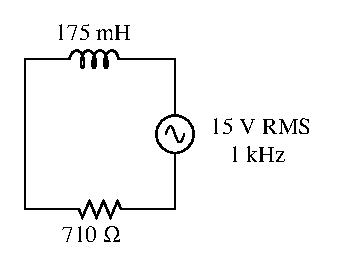
\includegraphics[width=15.5cm]{i01034x01.eps}$$

Beregn også faseforskyvning mellom $V_R$ og $V_{supply}$, samt mellom $V_L$ og $V_{supply}$.

\vfil

\underbar{file i01034}
\eject
%(END_QUESTION)





%(BEGIN_ANSWER)

Dette er en vurderingsoppgave -- ingen fasit eller hint oppgis!

%(END_ANSWER)





%(BEGIN_NOTES)

Stegvis metode og eksempelresultater:

$V_L = 12.60 \hbox{ V RMS}$

$V_R = 8.137 \hbox{ V RMS}$

$I = 11.46 \hbox{ mA RMS}$

Fase mellom $V_R$ og $V_{source}$ = 57.15$^{o}$

Fase mellom $V_L$ og $V_{source}$ = 32.85$^{o}$

%INDEX% Electronics review: AC reactance and impedance

%(END_NOTES)

